\begin{frame}{LVM -- управление логическими томами}
  \begin{center}
    \textbf{Структура LVM}
  \end{center}
  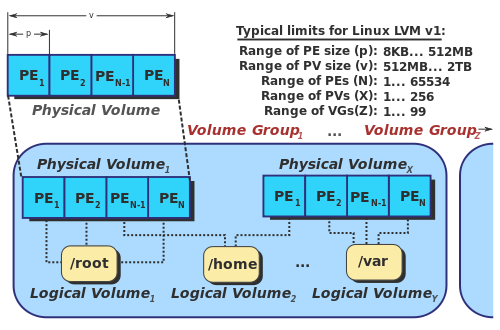
\includegraphics[width=0.7\textwidth]{../../slides/disk/LVM1-wiki.png}
\end{frame}

\begin{frame}{Преимущества LVM}
	\begin{itemize}
		\item Изменение размера
		\item Перемещение данных в активной системе
		\item Присвоение имен устройствам
		\item Чередование дисков
		\item Зеркалирование томов
		\item Снимки томов
	\end{itemize}
\end{frame}
 
\begin{frame}{LVM -- основные команды}
  \begin{itemize}
    \item Создание
      \begin{columns}
        \column{0.2\textwidth}
        \begin{itemize}
          \item pvcreate
        \end{itemize}
        \column{0.2\textwidth}
        \begin{itemize}
          \item vgcreate
        \end{itemize}
        \column{0.2\textwidth}
        \begin{itemize}
          \item lvcreate
        \end{itemize}
      \end{columns}
     \item Информация 
       \begin{columns}
         \column{0.2\textwidth}
         \begin{itemize}
           \item pvscan
           \item lvscan
           \item vgscan
		   \item lvmdiskscan
         \end{itemize}
         \column{0.2\textwidth}
         \begin{itemize}
           \item pvdisplay
           \item lvdisplay
           \item vgdisplay
		   \item[ ]
         \end{itemize}
         \column{0.2\textwidth}
         \begin{itemize}
           \item pvs
           \item lvs
           \item vgs
		   \item[ ]
         \end{itemize}
	 \end{columns}
      \item Манипулирование
        \begin{itemize}
          \item vgextend/vgreduce
          \item lvresize
          \item pvmove
          \item pvremove
         \end{itemize}
     \end{itemize}
    
\end{frame}

\begin{frame}{Упражнение: создание}
  \begin{enumerate}
    \item Создать 3 файла (200MB) и отобразить на {\tt /dev/loop[0-]}
	\item Найти устройства для работы с LVM {\tt lvmdiskscan}
	\item  {\tt pvcreate /dev/loop[0-2]}
    \item  {\tt pvscan, pvdisplay, pvs}
		\pause
    \item Создание группы томов {\tt vgcreate VG0 /dev/loop[0-2]}
    \item {\tt pvscan, vgscan, pvdisplay}
		\pause
    \item Создание логического тома {\tt lvcreate  -l 50\%VG -i 3 -n lv1 VG0}
	\item Создание файловой системы ext2 на {\tt /dev/VG0/lv1} и монтирование в {\tt /mnt/myfs}
	\end{enumerate}
\end{frame}

\begin{frame}{Изоляция процесса в Linux}
  \begin{center}
    \textbf{В порядке возрастания уровня изоляции}
  \end{center}
  \begin{enumerate}
    \item {\tt chroot}
    \item Linux containers (LXC)
    \item KVM/QEMU
  \end{enumerate}
\end{frame}

\begin{frame}{Упражнение: использование изоляции процесса}
  \begin{block}{chroot}
    \begin{enumerate}
      \item Выбрать из {\tt /media/nfs/pub/soft/linux/emulator/OpenVZ/precreated} систему по вкусу и распаковать {\tt tgz } файл в {\tt /mnt/myfs}
      \item Смонтировать proc и dev файловые системы в новом окружении {\tt /mnt/myfs} \\
		  Hints: {\tt procfs}, опция {\tt -\phantom{}-bind}
      \item {\tt chroot /mnt/myfs /bin/bash}
	  \item {\tt cat /etc/*release}
	  \item {\tt uname -a}
    \end{enumerate}
  \end{block}
\end{frame}

\begin{frame}{Упражнение: Создание снимка LVM}
  \begin{enumerate}
    \item  {\tt lvcreate -\phantom{}-snapshot -l 10\%VG -n snap /dev/VG0/lv1}
    \item  {\tt lvdisplay, lvs, lvscan}
	\item Смонтировать снимок в {\tt /mnt/snap}
		\pause
	\item Удалить директорию {\tt /mnt/snap/etc} или {\tt /mnt/myfs/etc}
	\item Отмонтировать снимок и оригинал\\
		Hint: помним про {\tt proc, dev}
		\pause
	\item Объединяем снимок с оригиналом {\tt lvconvert -\phantom{}-merge VG0/snap}
	\item Монтируем {\tt /dev/VG0/lv1} в {\tt /mnt/myfs} и проверяем изменения
  \end{enumerate}
\end{frame}

\begin{frame}{Упражнение: изменение размера VG}
  \begin{enumerate}
%	\item Отмонтировать {\tt /mnt/myfs}
	\item Создать еще один файл и отобразить его на {\tt loop3}
	\item Увеличиваем размер группы {\tt vgextend VG0 /dev/loop3}
		\pause
    \item  {\tt pvscan; pvmove /dev/loop0; pvscan}
    \item  {\tt vgreduce VG0 /dev/loop0; pvscan}
    \item  {\tt pvremove /dev/loop0; pvscan}
  \end{enumerate}
\end{frame}


